\documentclass[11pt,a4paper]{article}

\usepackage[T1]{fontenc}
\usepackage[russian]{babel}
\usepackage[utf8]{inputenc}
\usepackage{amsmath}
\usepackage{authblk}
\usepackage{extsizes}
\usepackage{graphicx}
\usepackage{mathptmx}
\usepackage{fullwidth}
\usepackage{svg}
\usepackage{amsmath}
\usepackage[backend=biber, style=numeric]{biblatex}
\usepackage{wrapfig}
\usepackage{geometry}

\geometry{
    a4paper,
    total={210mm,297mm},
    left=30mm,
    right=15mm,
    top=20mm,
    bottom=20mm,
}

\addbibresource{bibliography.bib}

\setlength{\parskip}{1em}

\title{Многоцелевой автономный малый беспилотный летательный аппарат}

\author{Кириенко П. С., Стойка Е. В., Кроль А. В.}

\affil{Zubax Robotics, г. Москва}

\date{}

\begin{document}

\maketitle

\section{Введение}

В настоящее время широкую популярность приобретают малые беспилотные летательные аппараты (МБПЛА) в различных прикладных задачах от аэрофотосъёмки до грузоперевозок. Мировой опыт эксплуатации различной авиации показывает, что безопасное и эффективное применение летательных аппаратов (ЛА) требует высокой квалификации оператора (пилота), и что именно оператор является наименее надёжным элементом в задаче пилотирования ЛА \cite{RiskManagementHandbookFAA, PlaneCrashInfo, HumanFactorsBoeing}. Кроме того, высокая стоимость рабочего времени квалифицированного оператора ограничивает множество задач, где использование МБПЛА показало бы экономическую эффективность \cite{DroneHire}.

В этой работе мы рассматриваем основные проблемы, связанные с разработкой адекватной системы управления (СУ) МБПЛА, способной максимально исключить человека из процесса пилотирования; предлагаем архитектуру программно-аппаратного обеспечения, и приводим реализации некоторых основных алгоритмов, выработанных к настоящему моменту в ходе продолжающегося исследования.

Ключевые отличия нашего подхода от используемых на сегодняшний день в индустрии следующие:

\begin{itemize}
    \item Использование компьютерного зрения для автономного счисления позиции, скорости и ориентации МБПЛА. Это обеспечивает надёжную оценку состояния даже при полной недоступности спутниковой навигационной системы (СНС).
    \item Использование компьютерного зрения для построения модели окружающего пространства. Это даёт СУ возможность безопасно пилотировать МБПЛА в сложных условиях без участия человека-оператора.
    \item Алгоритм комплексирования показаний различных сенсоров, способный корректно определять позицию, скорость и ориентацию БПЛА даже при недоступности измерений СНС и магнитного компаса.
\end{itemize}

В следующем разделе этой работы мы производим анализ задачи автоматизации процесса пилотирования МБПЛА с целью минимизации участия человека. Далее мы рассматриваем архитектуру программно-аппаратного обеспечения высокоавтономного МБПЛА, и затем приводим практическую реализацию двух ключевых компонентов такой системы: блока компьютерного зрения и надёжного алгоритма позиционирования.

\section{Анализ задачи}

Ниже приведён краткий список основных применений МБПЛА на сегодняшний день:

\begin{itemize}
    \item Грузоперевозки \cite{AmazonPrimeAir, DHLParcelcopter}.
    \item Аэрофотосъёмка, построение 3D моделей местности \cite{DroneMapper, MicrodronesAerialImagery}.
    \item Применение в СМИ (работа в городских условиях) \cite{DroneJournalism}.
    \item Поисково-спасательные операции \cite{SARDrones}.
    \item Спецоперации в городских или подобных условиях.
\end{itemize}

В контексте перечисленных применений можно выделить следующие ключевые проблемы современных технологий:

\begin{itemize}
    \item Cовременные автоматические СУ не в состоянии пилотировать МБПЛА в сложных условиях, таких как плотная городская застройка, ущелья, каньоны, леса, и т.п.
    \item Существующие решения требуют внимания оператора при выполнении манёвров около земли/препятствий, например, на этапе взлёта и посадки, даже если основная миссия может быть выполнена полностью автоматически.
    \item Основной причиной происшествий при эксплуатации ЛА является ошибка оператора (пилота) \cite{RiskManagementHandbookFAA, PlaneCrashInfo, HumanFactorsBoeing}.
    \item Можно предположить, что во многих приложениях системы с высокоавтономными МБПЛА будут иметь меньшие эксплуатационные расходы, чем управляемые человеком, так как один оператор сможет обслуживать большее количество аппаратов одновременно, либо получит возможность выполнять другие функции.
    \item Во многих странах (по меньшей мере, в странах ЕС \cite{EURPASFAQ} и Северной Америки \cite{FAAUAS}) коммерческое применение МБПЛА требует наличия лицензии оператора. Автоматически пилотируемый аппарат может, в теории, при наличии адекватного законодательства, избавить пользователей от необходимости найма лицензированых операторов.
\end{itemize}

Из вышесказанного можно вывести следующие требования к СУ высокоавтономного МБПЛА:

\begin{itemize}
    \item Осведомлённость об окружающем пространстве и безопасная навигация в нём.
    \item Использование алгоритмов оценки состояния, основанных на сенсорах различных принципов измерений, например: визуальная одометрия, СНС и ИНС.
    \item Отсутствие сильной зависимости от сенсоров, основой принципа действия которых являются измерения, чью надёжность и корректность сложно обеспечить. Примерами таких сенсоров являются: магнитный компас, датчик солнца, ультразвуковые или оптические дальномеры, и т.п.
    \item Способность безопасно завершить миссию при полной потере связи с наземным пунктом управления.
\end{itemize}

Данная работа решает следующие задачи из списка требований, приведённого выше (требования, которым этот список не удовлетворяет, являются предметом продолжающегося исследования):

\begin{itemize}
    \item Построение трёхмерной модели пространства вокруг МБПЛА средствами компьютерного зрения, что необходимо для безопасной навигации в нём.
    \item Алгоритм оценки состояния, основанный на измерениях системы компьютерного зрения, СНС и ИНС.
\end{itemize}

\section{Архитектура МБПЛА}

В качестве платформы был выбран лёгкий квадрокоптер полной массой <3 кг, оснащённый обычным промышленным компьютером Avalue ESM-QM77B-3612-A1R (платформа AMD64) под управлением операционной системы Ubuntu Server 64-bit и фреймворка Robotic Operating System (ROS) \cite{ROS}.

Согласно требованиям, изложенным выше, была разработана архитектура программно-аппаратного обеспечения, изображённая на рисунке \ref{fig:arch}.

\begin{figure}[!htbp]
    \centering
    \includesvg[width=1\textwidth]{Arch}
    \caption{\label{fig:arch}Архитектура программно-аппаратного обеспечения высокоавтономного МБПЛА.}
\end{figure}

Удалённый интерфейс оператора подключается к МБПЛА посредством беспроводного Wi-Fi соединения. Сенсоры и актуаторы подключается к компьютеру по шине UAVCAN \cite{UAVCAN}; исключение составляет стереокамера системы компьютерного зрения, основанная на 2-х камерах uEye UI-1249SE-C-HQ, подключенная посредством USB 2.0 HS. Модули стерео-отождествления, визуальной одометрии и построения трёхмерной модели местности формируют систему компьютерного зрения, рассмотренную детально далее в этом документе. Модуль определения позиции, скорости и ориентации так же описан в отдельной главе ниже. Контроллер позиции представляет собой простой каскадный ПИД-регулятор, уставкой которого является позиция и азимут, и выходные управляющие воздействия представлены в виде углов крена, тангажа и рысканья, которые затем передаются на контроллер ориентации на основе PX4 Pixhawk \cite{Pixhawk}. PX4 Pixhawk так же используется в качестве ИНС. Функции GPS/ГЛОНАСС приёмника возложены на модуль Zubax GNSS \cite{ZubaxGNSS}.

\newpage

\section{Система компьютерного зрения}

Система компьютерного зрения состоит из следующих компонентов:

\begin{itemize}
    \item Модуль визуальной одометрии на основе LIBVISO2 \cite{Geiger2011IV} вычисляет позицию и ориентацию камер относительно наблюдаемой сцены.
    \item Модуль стерео отождествления на основе ELAS \cite{Geiger10} использует стерео изображение для создания облака точек сцены, наблюдаемой стереокамерой.
    \item Модуль построения трёхмерной модели окружающего пространства использует облако точек и данные о позиции и ориентации для синтеза модели, представленной в виде октодерева \cite{rensselaer1980octree}. Метод оценки позиции и ориентации рассмотрен в соответствующей главе этого документа. Результирующее октодерево может быть использовано для планирования маршрута с учётом препятствий \cite{FraundorferHHLMTP12}, что, однако, выходит за рамки данной работы.
\end{itemize}

\begin{figure}[!htbp]
    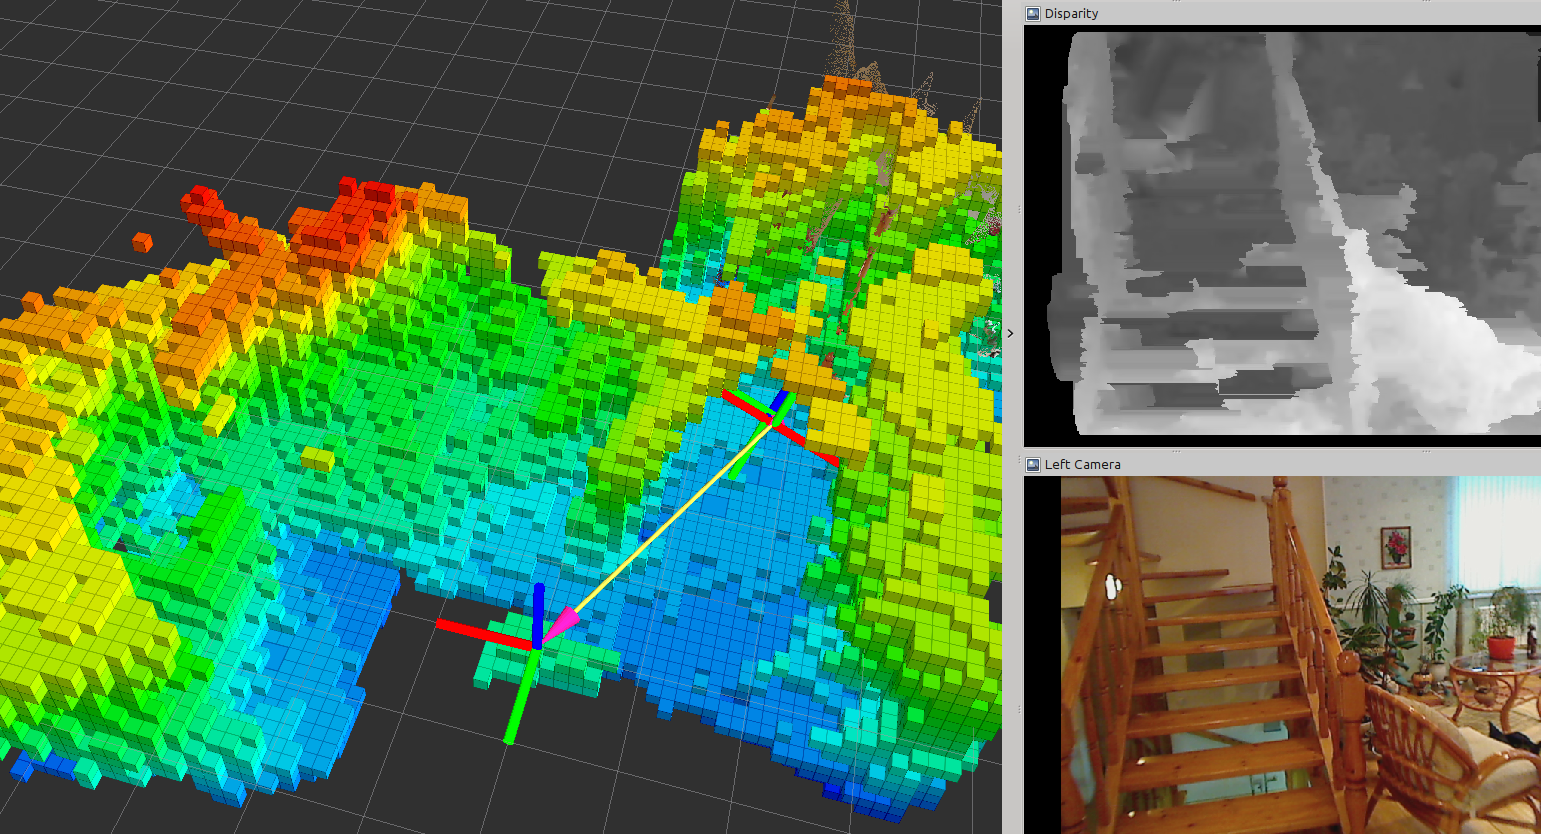
\includegraphics[width=1\textwidth]{octomap.png}
    \caption{\label{fig:octomap}Фрагмент трёхмерной модели помещения, построенный описанным выше методом. Оценка позиции и ориентации выполнялась по измерениям визуальной одометрии и ИНС. На изображении: слева - визуализация октодерева трёхмерной модели пространства, разрешение 15 см на воксель, цвет вокселя задаётся его высотой; справа-внизу - изображение левой камеры (изображение правой камеры не показано); справа-вверху - визуализация глубины сцены (ELAS).}
\end{figure}

\section{Алгоритм позиционирования}

Предлагаемый алгоритм позиционирования основывается на расширенном фильтре Калмана и решает задачу надёжной оценки состояния МБПЛА, включая позицию, скорость и ориентацию в пространстве. Отличительными особенностями предлагемого алгоритма являются:

\begin{itemize}
    \item Использование оценки позиции и ориентации на основе компьютерного зрения, что позволяет предотвратить накопление ошибки даже при длительной недоступности СНС.
    \item Способность алгоритма к надёжной оценке ориентации по азимуту на основе измерений СНС, что позволяет избежать применения сенсоров, основанных на менее надёжных принципах измерений, таких как магнитные компасы или датчики солнца.
\end{itemize}

Дальнейшее описание использует следующие определения:

\begin{itemize}
    \item $g$ - стандартное ускорение свободного падения на поверхности Земли.
    \item $q^*$ - комплексное сопряжённое $q$.
    \item $a \otimes b$ - произведение кватернионов $a$ и $b$ \cite{QuaternionsMadgwick}.
\end{itemize}

\subsection{Модель сенсоров}

Модель сенсоров основывается на следующих предположениях \cite{weiss2012vision}:

\begin{itemize}
    \item ИНС находится в центре масс МБПЛА, система координат (СК) ИНС совпадает с СК МБПЛА.
    \item Каждый сенсор имеет собственную СК, относительно которой выполняются измерения, и трансформация из локальной СК каждого сенсора в СК ИНС известна и постоянна.
    \item Измерения позиции, полученные от системы компьютерного зрения, выполнены в СК камеры.
    \item Измерения позиции, полученные от системы компьютерного зрения, подвержены медленному накоплению ошибки позиции и ориентации по мере движения МБПЛА.
\end{itemize}

Визуализация используемой модели систем координат приведена на иллюстрации \ref{fig:frames}, где:

\begin{itemize}
    \item $p_i^g$ - смещение антенны приёмника СНС относительно ИНС. Следует обратить внимание, что модель не предусматривает вращения антенны, т.к. этот параметр не влияет на наблюдаемые измерения этого сенсора.
    \item $p_i^c$ $q_i^c$ - смещение и поворот СК камеры относительно ИНС. Согласно принятому соглашению \cite{ROSFrames}, ось $z_c$ камеры совпадает с её оптической осью, ось $y_c$ направлена вниз, ось $x_c$ направлена вправо.
    \item $p_v^c$ $q_v^c$ - позиция и ориентация, согласно измерениям системы компьютерного зрения. Как было замечено выше, эти измерения подвержены медленному накоплению ошибки позиции и ориентации.
    \item $p_v^w$ $q_v^w$ - накопленная ошибка (смещение) оценки позиции и ориентации системой компьютерного зрения.
    \item $p_i^w$ $q_i^w$ - позиция и ориентация ИНС относительно глобальной СК.
\end{itemize}

\begin{figure}[!h]
    \centering
    \includesvg[width=0.7\textwidth]{frames}
    \caption{\label{fig:frames}Модель систем координат (СК).}
\end{figure}

\subsection{Вектор состояния}

Компоненты вектора состояния приведены в формуле \ref{eq:x} и детально рассмотрены ниже.

\begin{equation}
    \label{eq:x}
    x=\left(
    \begin{array}{c}
    p_w^i \\
    v_w^i \\
    q_w^i \\
    a \\
    w \\
    j_a \\
    j_w \\
    b_a \\
    b_w \\
    p_v^w \\
    q_v^w \\
    \end{array}
    \right)
\end{equation}

Компоненты вектора состояния:
\begin{itemize}
    \item $p_w^i$ - см. рис. \ref{fig:frames}.
    \item $v_w^i$ - скорость ИНС относительно глобальной СК.
    \item $q_w^i$ - см. рис. \ref{fig:frames}.
    \item $a$ - ускорение ИНС в ИСО.
    \item $w$ - угловая скорость ИНС в ИСО.
    \item $j_a$ - рывок ИНС в ИСО (первая производная ускорения) \cite{Kishore94}.
    \item $j_w$ - угловое ускорение ИНС в ИСО \cite{Kishore94}.
    \item $b_a$ - дрейф акселерометра ИНС.
    \item $b_w$ - дрейф ДУС ИНС.
    \item $p_v^w$ - см. рис. \ref{fig:frames}.
    \item $q_v^w$ - см. рис. \ref{fig:frames}.
\end{itemize}

Вращения в векторе состояния представлены в виде кватернионов поворота \cite{QuaternionsMadgwick}, линейные перемещения представлены в виде трёхмерных векторов, что в итоге порождает вектор состояния из 35 вещественных переменных. Состояние фильтра включает в себя производные позиции и ориентации высокого порядка, поскольку было показано преимущество подобного подхода в задачах определения состояния высокодинамических систем \cite{Kishore94}. Ошибка оценки состояния представлена согласно классическому подходу, в виде ковариационной матрицы $35 \times 35$.

Функция предсказания состояния $f(x,\text{$\Delta $t})$, где $\Delta t$ - интервал предсказания, приведена ниже.

\begin{equation}
    \label{eq:f}
    f(x,\text{$\Delta $t})=\left(
    \begin{array}{c}
    p_w^i+\text{$\Delta $t} v_w^i+\text{$\Delta $t}^2 qrot\left(a+\text{$\Delta $t} j_a,\left(q_w^i\right){}^*\right) \\
    v_w^i+\text{$\Delta $t} \text{ } qrot\left(a+\text{$\Delta $t} j_a,\left(q_w^i\right){}^*\right) \\
    q_w^i\otimes quaternion\left(j_w \text{$\Delta $t}^2+w \text{$\Delta $t}\right) \\
    a+\text{$\Delta $t} j_a \\
    w+\text{$\Delta $t} j_w \\
    j_a \\
    j_w \\
    b_a \\
    b_w \\
    p_v^w \\
    q_v^w \\
    \end{array}
    \right)
\end{equation}

Определение некоторых тривиальных функций, используемых в модели фильтра, приведено ниже \cite{QuaternionsMadgwick, QuaternionsNASA}.

\begin{equation}
    \label{eq:quaternion}
    quaternion(\phi ,\theta ,\psi )=\left(
    \begin{array}{c}
    w \\
    x \\
    y \\
    z \\
    \end{array}
    \right)=\left(
    \begin{array}{c}
    \cos \left(\frac{\theta }{2}\right) \cos \left(\frac{\phi }{2}\right) \cos \left(\frac{\psi }{2}\right)+\sin \left(\frac{\theta }{2}\right) \sin \left(\frac{\phi }{2}\right) \sin \left(\frac{\psi }{2}\right) \\
    \cos \left(\frac{\theta }{2}\right) \cos \left(\frac{\psi }{2}\right) \sin \left(\frac{\phi }{2}\right)-\cos \left(\frac{\phi }{2}\right) \sin \left(\frac{\theta }{2}\right) \sin \left(\frac{\psi }{2}\right) \\
    \cos \left(\frac{\phi }{2}\right) \cos \left(\frac{\psi }{2}\right) \sin \left(\frac{\theta }{2}\right)+\cos \left(\frac{\theta }{2}\right) \sin \left(\frac{\phi }{2}\right) \sin \left(\frac{\psi }{2}\right) \\
    \cos \left(\frac{\theta }{2}\right) \cos \left(\frac{\phi }{2}\right) \sin \left(\frac{\psi }{2}\right)-\cos \left(\frac{\psi }{2}\right) \sin \left(\frac{\theta }{2}\right) \sin \left(\frac{\phi }{2}\right) \\
    \end{array}
    \right)
\end{equation}

\begin{equation}
    \label{eq:euler}
    euler(w,x,y,z)=\left(
    \begin{array}{c}
    \tan ^{-1}\left(1-2 \left(x^2+y^2\right),2 (w x+y z)\right) \\
    \sin ^{-1}(2 (w y-x z)) \\
    \tan ^{-1}\left(1-2 \left(y^2+z^2\right),2 (x y+w z)\right) \\
    \end{array}
    \right)
\end{equation}

\begin{equation}
    \label{eq:qrot}
    qrot(\text{vec},q)=q\otimes \text{vec}\otimes q^*
\end{equation}

\subsection{Модель измерений}

В этой части приводятся уравнения предсказания измерений расширенного фильтра Калмана.

Функции предсказания измерений акселерометра и ДУС ИНС:

\begin{equation}
    h_{\text{acc}}(x)=qrot\left(\left(
    \begin{array}{c}
    0 \\
    0 \\
    g \\
    \end{array}
    \right),q_w^i\right)+b_a+a
\end{equation}

\begin{equation}
    h_{\text{gyro}}(x)=b_w+w
\end{equation}

Функции предсказания измерений позиции и скорости СНС:

\begin{equation}
    h_{\text{gnsspos}}(x)=p_w^i
\end{equation}

\begin{equation}
    h_{\text{gnssvel}}(x)=v_w^i
\end{equation}

Функции предсказания измерений позиции, скорости и ориентации, полученные от системы компьютерного зрения:

\begin{equation}
    h_{\text{vispos}}(x)=qrot\left(p_v^w,\left(q_v^w\right){}^*\right)+p_w^i
\end{equation}

\begin{equation}
    h_{\text{visvel}}(x)=qrot\left(v_w^i,\left(q_v^w\right){}^*\right)
\end{equation}

\begin{equation}
    h_{\text{visatt}}(x)=euler\left(q_w^i\otimes q_v^w\right)
\end{equation}

\subsection{Реализация}

Описанный выше расширенный фильтр Калмана реализован на языке C++ для системы Robotic Operating System (ROS) \cite{ROS} с использованием разработанного в рамках данного исследования инструмента синтеза исходного кода по высокоуровневому описанию уравнений фильтра. Процесс синтеза происходит следующим образом:

\begin{enumerate}
    \item Уравнения фильтра описываются на языке Wolfram Mathematica.
    \item Полученное описание используется для генерации исходного текста C++ класса вектора состояния фильтра, для чего применяется разработанная в рамках данного исследования утилита.
    \item Сгенерированнй класс вектора состояния используется C++ приложением, где реализуются низкоуровневые задачи обработки измерений и обновления состояния фильтра.
\end{enumerate}

Исходные тексты описанных компонентов можно найти по URL: \url{https://github.com/Zubax/zubax_posekf}.

\subsection{Результаты}

Тестирование фильтра выполнялось с использованием свободно доступных тестовых данных CAMPUS-0L и CAMPUS-2L \cite{blanco2009cor}.

(...)

\section{Заключение}



\nocite{*}
\begin{fullwidth}
\printbibliography
\end{fullwidth}

\end{document}
